\documentclass[]{standalone}
\usepackage{tikz}
\usetikzlibrary{shapes,arrows,calc,positioning}
\usepackage{amsmath} % for dfrac
\usepackage{comment}
\usepackage{calc}

% Decision
\tikzstyle{decision} = [diamond, aspect=1.8, minimum width=2cm, minimum height=1cm, text centered, text width=2cm, draw=black]

% definition of basic block
\tikzset{
    block/.style = {draw, rectangle,
        minimum height=1.2cm,
        minimum width=2cm},
    cblock/.style = {draw, circle,
    	minimum height=1.2cm,
    	minimum width=2cm},
    input/.style = {coordinate,node distance=1cm},
    output/.style = {coordinate,node distance=1cm},
    sum/.style = {draw, circle, node distance=1cm},
}

% definition of saturation block
\tikzset{% from https://tex.stackexchange.com/questions/161075/saturation-block
  saturation block/.style={%
    draw, 
    path picture={
      % Get the width and height of the path picture node
      \pgfpointdiff{\pgfpointanchor{path picture bounding box}{north east}}%
        {\pgfpointanchor{path picture bounding box}{south west}}
      \pgfgetlastxy\x\y
      % Scale the x and y vectors so that the range
      % -1 to 1 is slightly shorter than the size of the node
      \tikzset{x=\x*.4, y=\y*.4}
      %
      % Draw annotation
      \draw (-1,0) -- (1,0) (0,-1) -- (0,1); 
      \draw (-1,-.7) -- (-.6,-.7) -- (.6,.7) -- (1,.7);
    }
  }
}
\tikzset{% from https://tex.stackexchange.com/questions/161075/saturation-block
  deadband block/.style={%
    draw, 
    path picture={
      % Get the width and height of the path picture node
      \pgfpointdiff{\pgfpointanchor{path picture bounding box}{north east}}%
        {\pgfpointanchor{path picture bounding box}{south west}}
      \pgfgetlastxy\x\y
      % Scale the x and y vectors so that the range
      % -1 to 1 is slightly shorter than the size of the node
      \tikzset{x=\x*.4, y=\y*.4}
      %
      % Draw annotation
      \draw (-1,0) -- (1,0) (0,-1) -- (0,1);  % axis
      \draw (-1,1) -- (-.3,.3) -- (-.3,0) -- (.3,0) -- (.3,-.3) -- (1,-1);
	  %\draw (-.3,.3) -- (.3,-.3) ;
    }
  }
}

\begin{document}
	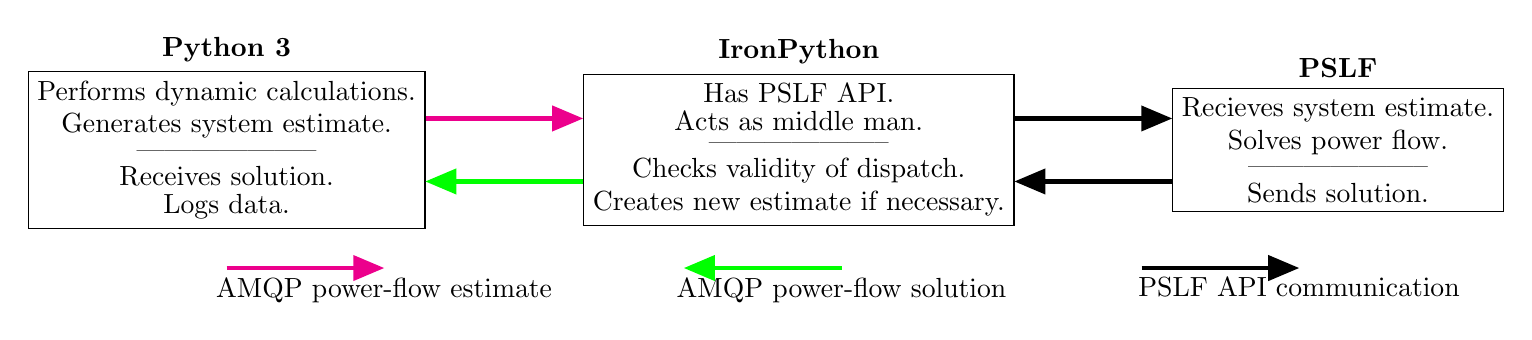
\begin{tikzpicture}[auto, node distance=.5cm,>=triangle 45]
		
		
		% py3
		\node [block, label=\textbf{Python 3}] (PY3) {
		%\begin{minipage}{2in}
			\shortstack{
			Performs dynamic calculations.\\
			Generates system estimate.\\
			--------------------\\
			Receives solution.\\
			Logs data.}
		%\end{minipage}
		};
		
		% ipy
		\node [block, right=2cm of PY3,label=\textbf{IronPython} ] (IPY) {
			%\begin{minipage}{2in}
				\shortstack{
				Has PSLF API.\\
				Acts as middle man.\\
				--------------------\\
				Checks validity of dispatch.\\
				Creates new estimate if necessary.}
			%\end{minipage}
	};
		
		% pslf
		\node [block, right=2cm of IPY, label=\textbf{PSLF} ] (PSLF) {
			%\begin{minipage}{2in}
			\shortstack{
			Recieves system estimate.\\
			Solves power flow.\\
			--------------------\\
			Sends solution.}
			%\end{minipage}	
	};

% 'legend'
\coordinate[below=0.5cm of PY3] (est left);
\coordinate[right=2cm of est left,label={[anchor=north]above:AMQP power-flow estimate}] (est right);	
\draw [->, magenta, ultra thick] (est left) -- (est right);	

\coordinate[right=1.5in of est right] (soln left);
\coordinate[right=2cm of soln left, label={[anchor=north]above:AMQP power-flow solution}] (soln right);	
\draw [<-, green, ultra thick] (soln left) -- (soln right);	

\coordinate[right=1.5in of soln right] (api left);
\coordinate[right=2cm of api left, label={[anchor=north]above:PSLF API communication}] (api right);	
\draw [->, black, ultra thick] (api left) -- (api right);	



\draw [->, magenta, ultra thick]  ($(PY3.east)+ (0,0.4)$) --  ($(IPY.west)+ (0,0.4)$);
\draw [->,black, ultra thick] ($(IPY.east)+ (0,0.4)$) -- ($(PSLF.west)+ (0,0.4)$);

\draw [<-, green, ultra thick]  ($(PY3.east)+ (0,-0.4)$) --  ($(IPY.west)+ (0,-0.4)$);
\draw [<-,black, ultra thick] ($(IPY.east)+ (0,-0.4)$) -- ($(PSLF.west)+ (0,-0.4)$);
		
		%\draw[->,green, ultra thick] (PSLF.south)  .. controls +(down:1cm) and +(down:1cm) .. ($(IPY.south)+ (0.5,0)$);
		%\draw[->,green, ultra thick] ($(IPY.south)+ (-0.5,0)$)  .. controls +(down:1cm) and +(down:1cm)		.. (PY3.south);
		
		% pf convergence bad
		%\draw [->] (simOver) --  node[anchor=east] {Yes} (pythonoutput);
		%\draw (simOver.west) -- node[anchor=north] {No} ($(simOver.west) + (-2,0)$);
		%\draw [->] ($(simOver.west) + (-2,0)$) |-  (pythonloop1.west);

	\end{tikzpicture} 
\end{document}